\documentclass[a4paper,10pt]{article}
\usepackage[utf8]{inputenc}
\usepackage{graphicx}
\usepackage{amsmath}
\usepackage{amssymb}
\usepackage{amsthm}
\usepackage{booktabs}
\usepackage{caption}
\usepackage{geometry}
%\usepackage{hyperref}
\usepackage{makeidx}
\usepackage{microtype}
\usepackage{subfig}
\usepackage{tabularx}
\usepackage{url}
\usepackage{varioref}
\usepackage{xcolor}
\usepackage{multicol}
\usepackage[italian]{babel}
\usepackage{mathtools}
\usepackage{fancyhdr}
\pagestyle{fancy}

\addto\captionsenglish{
  \renewcommand{\contentsname}%
    {Indice}%
}


\title{Laboratorio I: Pendolo semplice\\ Analisi della dipendenza del periodo dalla massa, ampiezza e lunghezza\\
\begin{large}
Dipartimento di Fisica E.Fermi - Università di Pisa
\end{large}}

\author{Di Ubaldo Gabriele}
\date{}
\begin{document}

\maketitle


%%%%%%%%%%%%%%%%%%%%%%%%%%%%%%%%%%%%%%%%%%%%%%%%%%%%%%%%%%%%%%%%%%%%%%%%%%%%%%%%%%%%%%%%%%%%%%%%%%%%%%%%%%%%%%%%%%%%%%%%%%%%%%%%%%%%%%%%%%%%%%%%%%%%%%%%%%%%%%%%%%%%%%%%%%
\section{Introduzione}
\subsection{Teoria}
\textbf{Obiettivo:} Studiare il periodo del pendolo semplice e determinare se esso sia legato proporzionalmente al raggio di oscillazzione, alla massa oscillante e 
alla ampiezza. 
Il periodo del pendolo per piccole oscillazioni è dato dalla formula:
\begin{equation}\label{pendolo}
T=2\pi\sqrt{\frac{l}{g}}
\end{equation}
Ottenuta sviluppando al primo ordine $\sin\theta=\theta$. Il periodo quadro dovrebbe dipendere linearmente dalla lunghezza e non dipendere in alcun modo da massa o dall'ampiezza iniziale.

\subsection{Apparato sperimentale}
\begin{itemize}
\item{Pendolo semplice fissato alla parete con meccanismo per variare il perno}
\item{Cronometro di risoluzione $0.01s$}
\item{Bilancia di precisione di risoluzione $0.001g$}
\item{Metro a nastro di risoluzione $1mm$}
\item{Calibro ventesimale di risoluzione $0.05 mm$}
\item{Tre pesetti di masse: $m_1=85.967g; m_2=53.107g; m_3=31.175g$}
\item{Anello per appendere i solidi di massa $m_A=0.459g$ e diametro $d_A=10mm$}
\end{itemize}

%%%%%%%%%%%%%%%%%%%%%%%%%%%%%%%%%%%%%%%%%%%%%%%%%%%%%%%%%%%%%%%%%%%%%%%%%%%%%%%%%%%%%%%%%%%%%%%%%%%%%%%%%%%%%%%%%%%%%%%%%%%%%%%%%%%%%%%%%%%%%%%%%%%%%%%%%%%%%%%%%%%%%%%%%%%%%%%%%
\section{Esperimento}
\footnote{Tutte le misure prese sono da intendersi con il corrispondente errore dato dalla risoluzione dello strumento}
Per eliminare possibili errori sistematici (parallassi) abbiamo mantenuto costante la distanza del pendolo dalla parete  $d=54mm$ e abbiamo fatto oscillare il pendolo in un piano parallelo alla parete e perpendicolare al suolo.
Il valore di $\theta$  è stato determinato prendendo un cateto arbitrariamente piccolo (il più grande è $c=50mm$), così da poter approssimare $\sin{\theta}\simeq{\theta}$, e utilizzando $\arcsin({\frac{c}{l}})$. 
L'approssimazione è valida in quanto per l'angolo da noi scelto si ha $\sin{0.096}=0.0958\dots$
La propagazione dell'errore per le ampiezze è stata fatta tramite derivate parziali:
\begin{equation}
\Delta\theta=c/{l^2 }\frac{1}{1+(c/l)^2}\Delta l+ 1/l\frac{1}{1+(c/l)^2}\Delta c
\end{equation}

\subsection{Dipendenza dalla massa $m$ }
Durante l'esperimento manteniamo costanti la lunghezza $l=l_p+l_A+l_m=503\pm 1mm$ e l'angolo $\theta=0,096\pm0,002 rad$ del pendolo attraverso dei segni sulla carta millimetrata posta dietro il pendolo.
Sono state effettuate 5 misurazioni di 10 oscillazioni ognuna($T=10t$) per 3 masse.
Al variare della massa campione, è stato necessario modificare il punto di applicazione del pendolo, così come la lunghezza del filo,
per mantenere costanti l'angolo e la lunghezza
\\I risultati ottenuti sono descritti dalla seguente tabella:\\

\begin{table}[!htb]
\centering
\caption{Massa-periodo}
\label{my-label}
\begin{tabular}{c|ccccc|l}
$m(g)$ & \multicolumn{5}{c|}{$T(s)$}           & $T_m(s)$       \\ \hline
85.967 & 14.15 & 14.25 & 14.29 & 14.17 & 14.24 & $14.22\pm0.05$ \\
53.107 & 14.18 & 14.32 & 14.13 & 14.22 & 14.28 & $14.23\pm0.07$ \\
31.175 & 14.31 & 14.20 & 14.27 & 14.19 & 14.16 & $14.23\pm0.06$
\end{tabular}
\end{table}

\begin {figure}[!htb]
\begin{center}
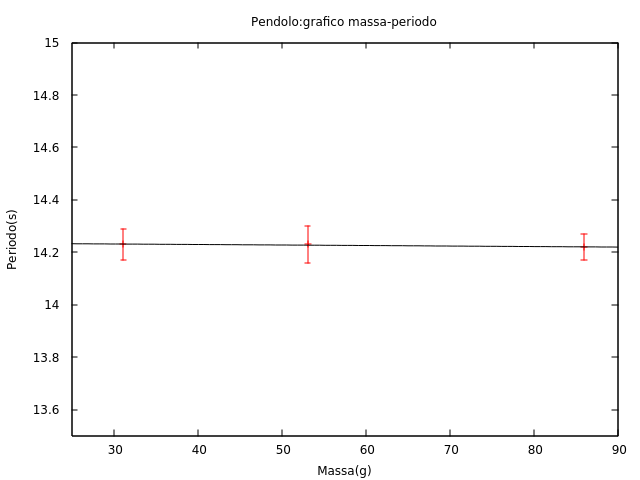
\includegraphics[width=10cm]{/home/zerch/Documents/UNIPI/LAB1/1Pendolo/grafici/graf-m-T.png}
\end{center}
\end {figure}
Abbiamo fatto un fit con Gnuplot (algoritmo di Marquardt-Levenberg) con i seguenti risultati:
\begin{equation}
\chi2=0.0024 \quad \chi2_r=0.0024 \quad a=-0.0002\pm35.36\% b=14.24\pm9.032\%
\end{equation}
Questi risultati confermano l'indipendenza del periodo dalla massa come predetto dal modello fisico.

\subsection{Dipendenza dall'ampiezza $\theta$}
Abbiamo mantenuto costanti la lunghezza $l=503\pm1mm$ e la massa $m=m_1+m_A=86,426\pm2 g$
Sono state effettuate 5 misurazioni di 10 oscillazioni ognuna($T=10t$) per 5 angoli diversi.
I risultati ottenuti sono descritti dalla seguente tabella:
\begin{table}[!htb]
\centering
\caption{Ampiezza-periodo}
\label{my-label}
\begin{tabular}{c|ccccc|c}
$\theta(rad)$ & \multicolumn{5}{c|}{$T(s)$}           & $T_m(s)$       \\ \hline
0.174         & 14.25 & 14.28 & 14.35 & 14.17 & 14.14 & $14.24\pm0.08$ \\
0.349         & 14.19 & 14.34 & 14.16 & 14.26 & 14.28 & $14.25\pm0.06$ \\
0.523         & 14.33 & 14.20 & 14.18 & 14.31 & 14.25 & $14.25\pm0.06$ \\
0.698         & 14.34 & 14.22 & 14.26 & 14.28 & 14.25 & $14.27\pm0.04$ \\
0.872         & 14.23 & 14.16 & 14.24 & 14.19 & 14.31 & $14.23\pm0.05$
\end{tabular}
\end{table}

\begin {figure}[!htb]
\begin{center}
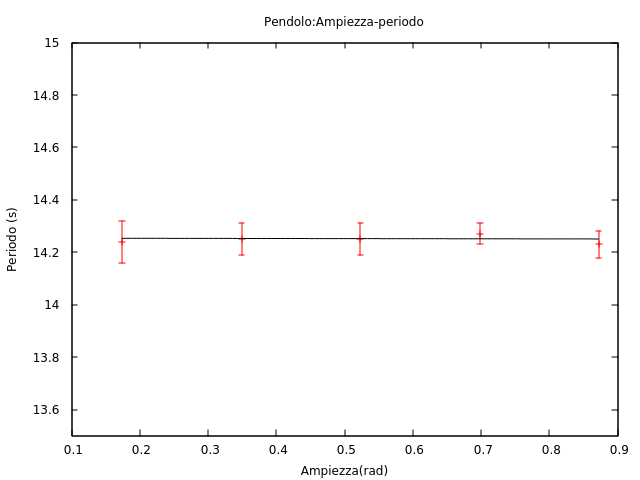
\includegraphics[width=10cm]{/home/zerch/Documents/UNIPI/LAB1/1Pendolo/grafici/graf-theta-T.png}
\end{center}
\end {figure}

I risultati del fit sono:
\begin{equation}
\chi2=0.42 \quad \chi2_r=0.14 \quad a=-0.004\pm1112\% \quad b=14.25\pm0.2\%
\end{equation}
Dal $\chi^2$ possiamo confermare che come predetto dal nostro modello fisico, il periodo è indipendente dall'ampiezza. L'altissimo errore sul coefficiente angolare $a$ potrebbe sembrare negativo ma ha senso che sia così poichè $a$ deve essere prossimo a 0 e quindi è normale che l'errore relativo sia altissimo.



\subsection{Dipendenza dalla lunghezza $l$}
Manteniamo costanti la massa $m=m_1+m_A=86,426\pm2 g$ e l'ampiezza $\theta=0,096\pm0,002 rad$.
Sono state effettuate 5 misurazioni di 10 oscillazioni ognuna($T=10t$) per 5 angoli diversi.
\\I risultati ottenuti sono descritti dalla seguente tabella:\\

\begin{table}[!htb]
\centering
\caption{Lunghezza-periodo}
\label{my-label}
\begin{tabular}{c|ccccc|c}
$l(mm)$ & \multicolumn{5}{c|}{$T(s)$}           & $T_m(s)$       \\ \hline
519     & 14.48 & 14.62 & 14.54 & 14.34 & 14.38 & $14.47\pm0.1$  \\
582     & 15.35 & 15.42 & 15.21 & 15.24 & 15.45 & $15.33\pm0.1$  \\
662     & 16.40 & 16.22 & 16.36 & 16.27 & 16.44 & $16.34\pm0.08$ \\
734     & 17.21 & 17.25 & 17.15 & 17.09 & 17.28 & $17.20\pm0.07$ \\
786     & 17.81 & 17.71 & 17.69 & 17.85 & 17.88 & $17.79\pm0.07$
\end{tabular}
\end{table}

\begin {figure}[!htb]
\begin{center}
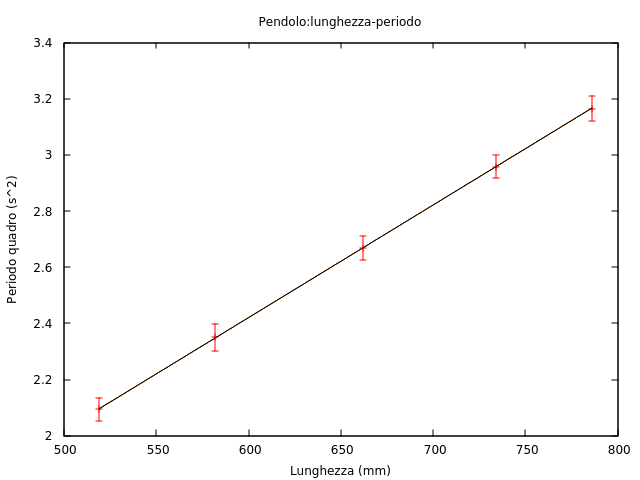
\includegraphics[width=10cm]{/home/zerch/Documents/UNIPI/LAB1/1Pendolo/grafici/graf-l-T.png}
\end{center}
\end {figure}
Abbiamo fatto un fit lineare tra la lunghezza e il periodo quadro ottenendo i seguenti risultati:
\begin{equation}
\chi^2= 0.005 \quad \chi^2_r=0.0017 \quad a=0.004\pm0.3\% \quad b=0.014\pm 39\%
\end{equation}
Il valore del $\chi^2$ conferma la validità del modello fisico. L'intercettà è compatibile con 0 come indica $T^2=\frac{4\pi^2}{g}l$ e dal coefficiente angolare possiamo stimare $g$.
\begin{equation}
g=9.84\pm0.02 m/s^2
\end{equation}
Valore molto vicino a quello di Pisa ma non compatibile, probabilmente per ua sottostima dell'errore.


\pagebreak
\section{Conclusione}
In base ai risultati ottenuti dagli esperimenti, si può assumere la dipendenza del periodo del pendolo solo da $l$ (quadratica), escludendo,quindi, $m$ e $\theta$.

\end{document}







